% Tiêu đề đầu trang
\begin{flushright}
{\textsf{\textbf{\footnotesize MỤC 2.8}}\hspace{1.2em}\textsf{\footnotesize Đạo hàm như một hàm số}}\hspace{2em}{\textsf{\textbf{\large 159}}}
\end{flushright}
\vspace{12pt}

% Khối 1: Lề trái đặt Hình 6, Cột chính đặt Đoạn 1
\noindent
\makebox[0pt][r]{%
  \begin{minipage}[t]{125pt}
    \vspace{0pt}%
    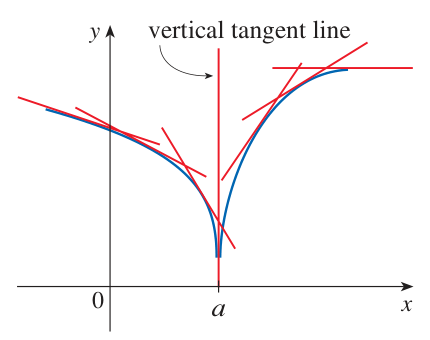
\includegraphics[width=\linewidth]{images/p0194_fig1.png}\\[3pt]
    \textsf{\textbf{\small HÌNH 6}}
  \end{minipage}\hspace{20pt}%
}%\noindent
Một khả năng thứ ba là đường cong có một \textbf{tiếp tuyến thẳng đứng} khi $x = a$; tức là, $f$ liên tục tại $a$ và
\[
\lim_{x \to a} |f'(x)| = \infty
\]
Điều này có nghĩa là các tiếp tuyến ngày càng dốc hơn khi $x \to a$. Hình 6 minh họa một trường hợp điều này có thể xảy ra; Hình 7(c) minh họa một trường hợp khác. Hình 7 mô tả ba khả năng mà chúng ta đã thảo luận.

\vspace{8pt}

% Khối 2: Lề trái đặt Chú thích Hình 7 dóng hàng đáy, Cột chính đặt Hình 7
\noindent
\makebox[0pt][r]{%
  \begin{minipage}[b]{125pt}
    \raggedright
    \textsf{\textbf{\small HÌNH 7}}\\[2pt]
    {\small Ba trường hợp để $f$ không\\khả vi tại $a$\par}
    \vspace{2pt}
  \end{minipage}\hspace{20pt}%
}%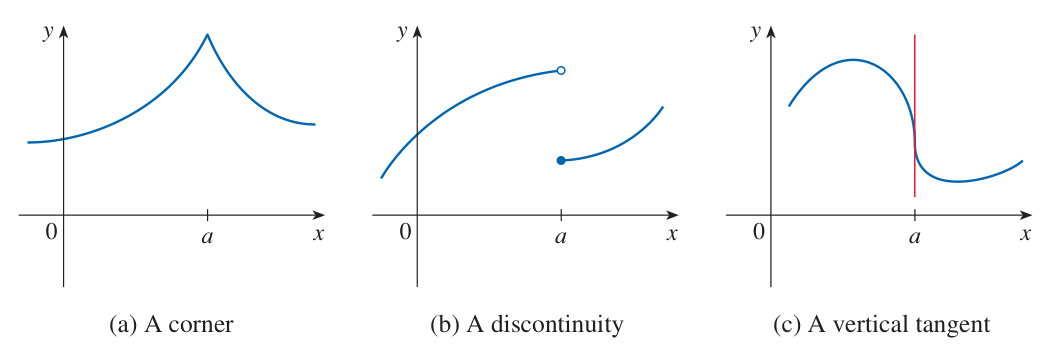
\includegraphics[width=\linewidth]{images/p0194_fig2.png}

\vspace{10pt}

% Đoạn 2: Giới thiệu tính khả vi qua phóng to đồ thị
Máy tính bỏ túi vẽ đồ thị hoặc máy vi tính cung cấp một cách khác để xem xét tính khả vi. Nếu $f$ khả vi tại $a$, thì khi chúng ta phóng to về phía điểm $(a, f(a))$, đồ thị sẽ thẳng dần ra và trông ngày càng giống một đường thẳng. (Xem Hình 8. Chúng ta đã thấy một ví dụ cụ thể về điều này trong Hình 2.7.2.) Nhưng cho dù chúng ta có phóng to bao nhiêu lần về phía một điểm như trong các Hình 6 và 7(a), chúng ta cũng không thể loại bỏ điểm nhọn hoặc điểm góc (xem Hình 9).

\vspace{10pt}

% Khối 3: Hình 8 và Hình 9 đặt song song
\noindent
\begin{minipage}[t]{0.48\linewidth}
  \centering
  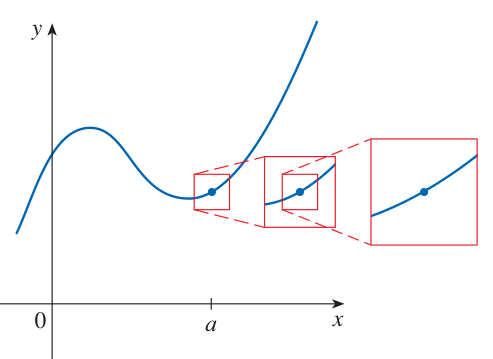
\includegraphics[width=\linewidth]{images/p0194_fig3.png}\\[4pt]
  \raggedright
  \textsf{\textbf{\small HÌNH 8}}\\[1pt]
  {\small $f$ khả vi tại $a$.}
\end{minipage}\hfill
\begin{minipage}[t]{0.48\linewidth}
  \centering
  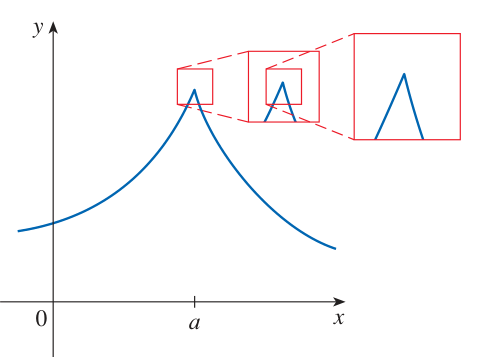
\includegraphics[width=\linewidth]{images/p0194_fig4.png}\\[4pt]
  \raggedright
  \textsf{\textbf{\small HÌNH 9}}\\[1pt]
  {\small $f$ không khả vi tại $a$.}
\end{minipage}

\vspace{14pt}

% Mục: Đạo hàm cấp cao
\noindent
\textcolor{stewartblue}{\rule{6pt}{6pt}}\hspace{0.5em}{\textsf{\textbf{\large Đạo hàm cấp cao}}}\\[5pt]
\noindent
Nếu $f$ là một hàm số khả vi, thì đạo hàm $f'$ của nó cũng là một hàm số, do đó $f'$ có thể có đạo hàm của riêng nó, ký hiệu là $(f')' = f''$. Hàm số mới $f''$ này được gọi là \textbf{đạo hàm cấp hai} của $f$ vì nó là đạo hàm của đạo hàm của $f$. Sử dụng ký hiệu Leibniz, ta viết đạo hàm cấp hai của $y = f(x)$ là

\[
\textcolor{stewartcyan}{\underbrace{\textcolor{black}{\frac{d}{dx}}}_{\substack{\text{\textsf{\scriptsize đạo hàm}}\\\text{\textsf{\scriptsize của}}}}}
\;
\textcolor{stewartcyan}{\underbrace{\textcolor{black}{\left(\frac{dy}{dx}\right)}}_{\substack{\text{\textsf{\scriptsize đạo hàm}}\\\text{\textsf{\scriptsize cấp một}}}}}
\;=\;
\textcolor{stewartcyan}{\underbrace{\textcolor{black}{\frac{d^2y}{dx^2}}}_{\substack{\text{\textsf{\scriptsize đạo hàm}}\\\text{\textsf{\scriptsize cấp hai}}}}}
\]

\vfill
\begin{center}
{\fontsize{5.5}{6.5}\selectfont\color{copyrightgray}
Copyright 2021 Cengage Learning. All Rights Reserved. May not be copied, scanned, or duplicated, in whole or in part. WCN 02-200-203\\Chỉ lưu hành nội bộ phục vụ mục đích học tập và nghiên cứu giảng dạy.}
\end{center}
